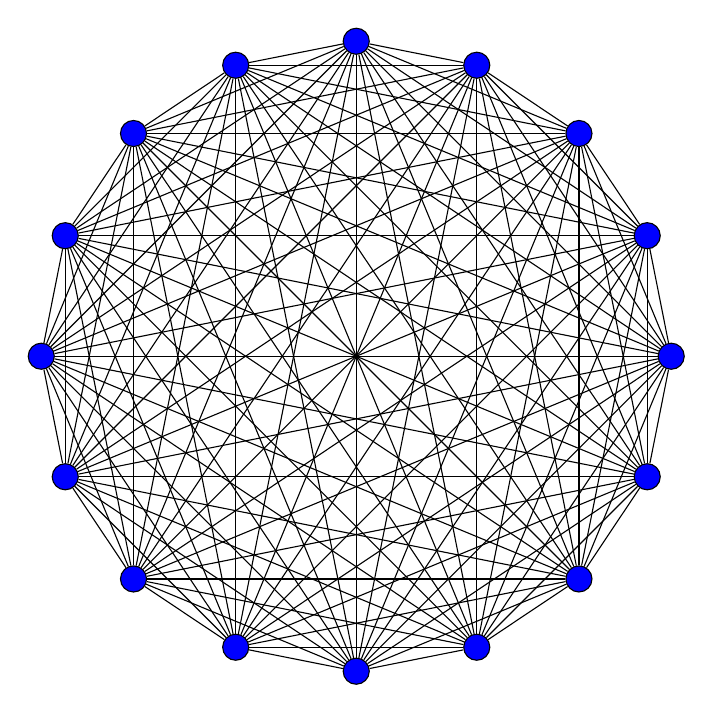
\begin{tikzpicture}
    \foreach \i in {1,...,16} {
      \node[draw, fill=blue, circle, minimum size=6pt] (v\i) at ({360/16 * (\i-1)}:4) {};
    }
    
    \foreach \i in {1,...,16} {
      \foreach \j in {1,...,16} {
        \ifnum\i<\j
          \draw (v\i) -- (v\j);
        \fi
      }
    }
    
  \end{tikzpicture}